\documentclass{article}
\usepackage[utf8]{inputenc}
\usepackage[spanish]{babel}
\usepackage{graphicx}	%Si se quiere compilar con las imagenes
% \usepackage[draft]{graphicx}	%Si NO se quiere compilar con las imagenes porque tarda mucho
\usepackage{graphics, float, fancyhdr, titling, caption, subcaption}
\usepackage{listings}
\usepackage[a4paper, total={6in, 9.5in}]{geometry}
\usepackage{fancyhdr}
\usepackage{hyperref}   %para que funcione addcontentsline debe ser la ultima que se cargue
\usepackage{amsmath}
%\setcounter{secnumdepth}{-2}       %Poner solo esto si no se quieren numero delante de las secciones y niveles inferiores.

\renewcommand{\footrulewidth}{0.4pt}
\title{

\includegraphics[width=1.75in]{imagenes/UGR-Logo.png} \\
\vspace*{1in}
\textbf{Memoria de la práctica 3} \\
Animación por Ordenador \\
\vspace*{0.5in}}
\author{Andrés Merlo Trujillo \\
andresmerlo@correo.ugr.es \\
77147239H \\ 
\vspace*{0.5in} \\
E.T.S. de Ingenierías Informática y de Telecomunicación \\
\textbf{Universidad de Granada}} \date{\today}

\hypersetup{
    colorlinks=true,
    linkcolor=black,
    citecolor=black
}

\renewcommand\maketitlehooka{\null\mbox{}\vfill}
\renewcommand\maketitlehookd{\vfill\null}

\begin{document}
\begin{titlingpage}
\maketitle
\end{titlingpage}

\tableofcontents

\newpage

\pagestyle{fancy}   %a partir de comienza el header (se salta el indice y portada)
\fancyhead[L]{Andrés Merlo Trujillo}
\fancyhead[R]{Animación por Ordenador}
%\section{Ejercicio 1}
%\begin{figure}[H]
%    \centering
%    \includegraphics[width=\textwidth]{imagenes/passwdfile.png}
%    \vspace{10pt}
%    \footnotesize{Fuente: https://...}
%\end{figure}

% \begin{figure}[H]
%     \centering 
% 	\begin{subfigure}[t]{0.48\textwidth}
% 	    \centering
% 	    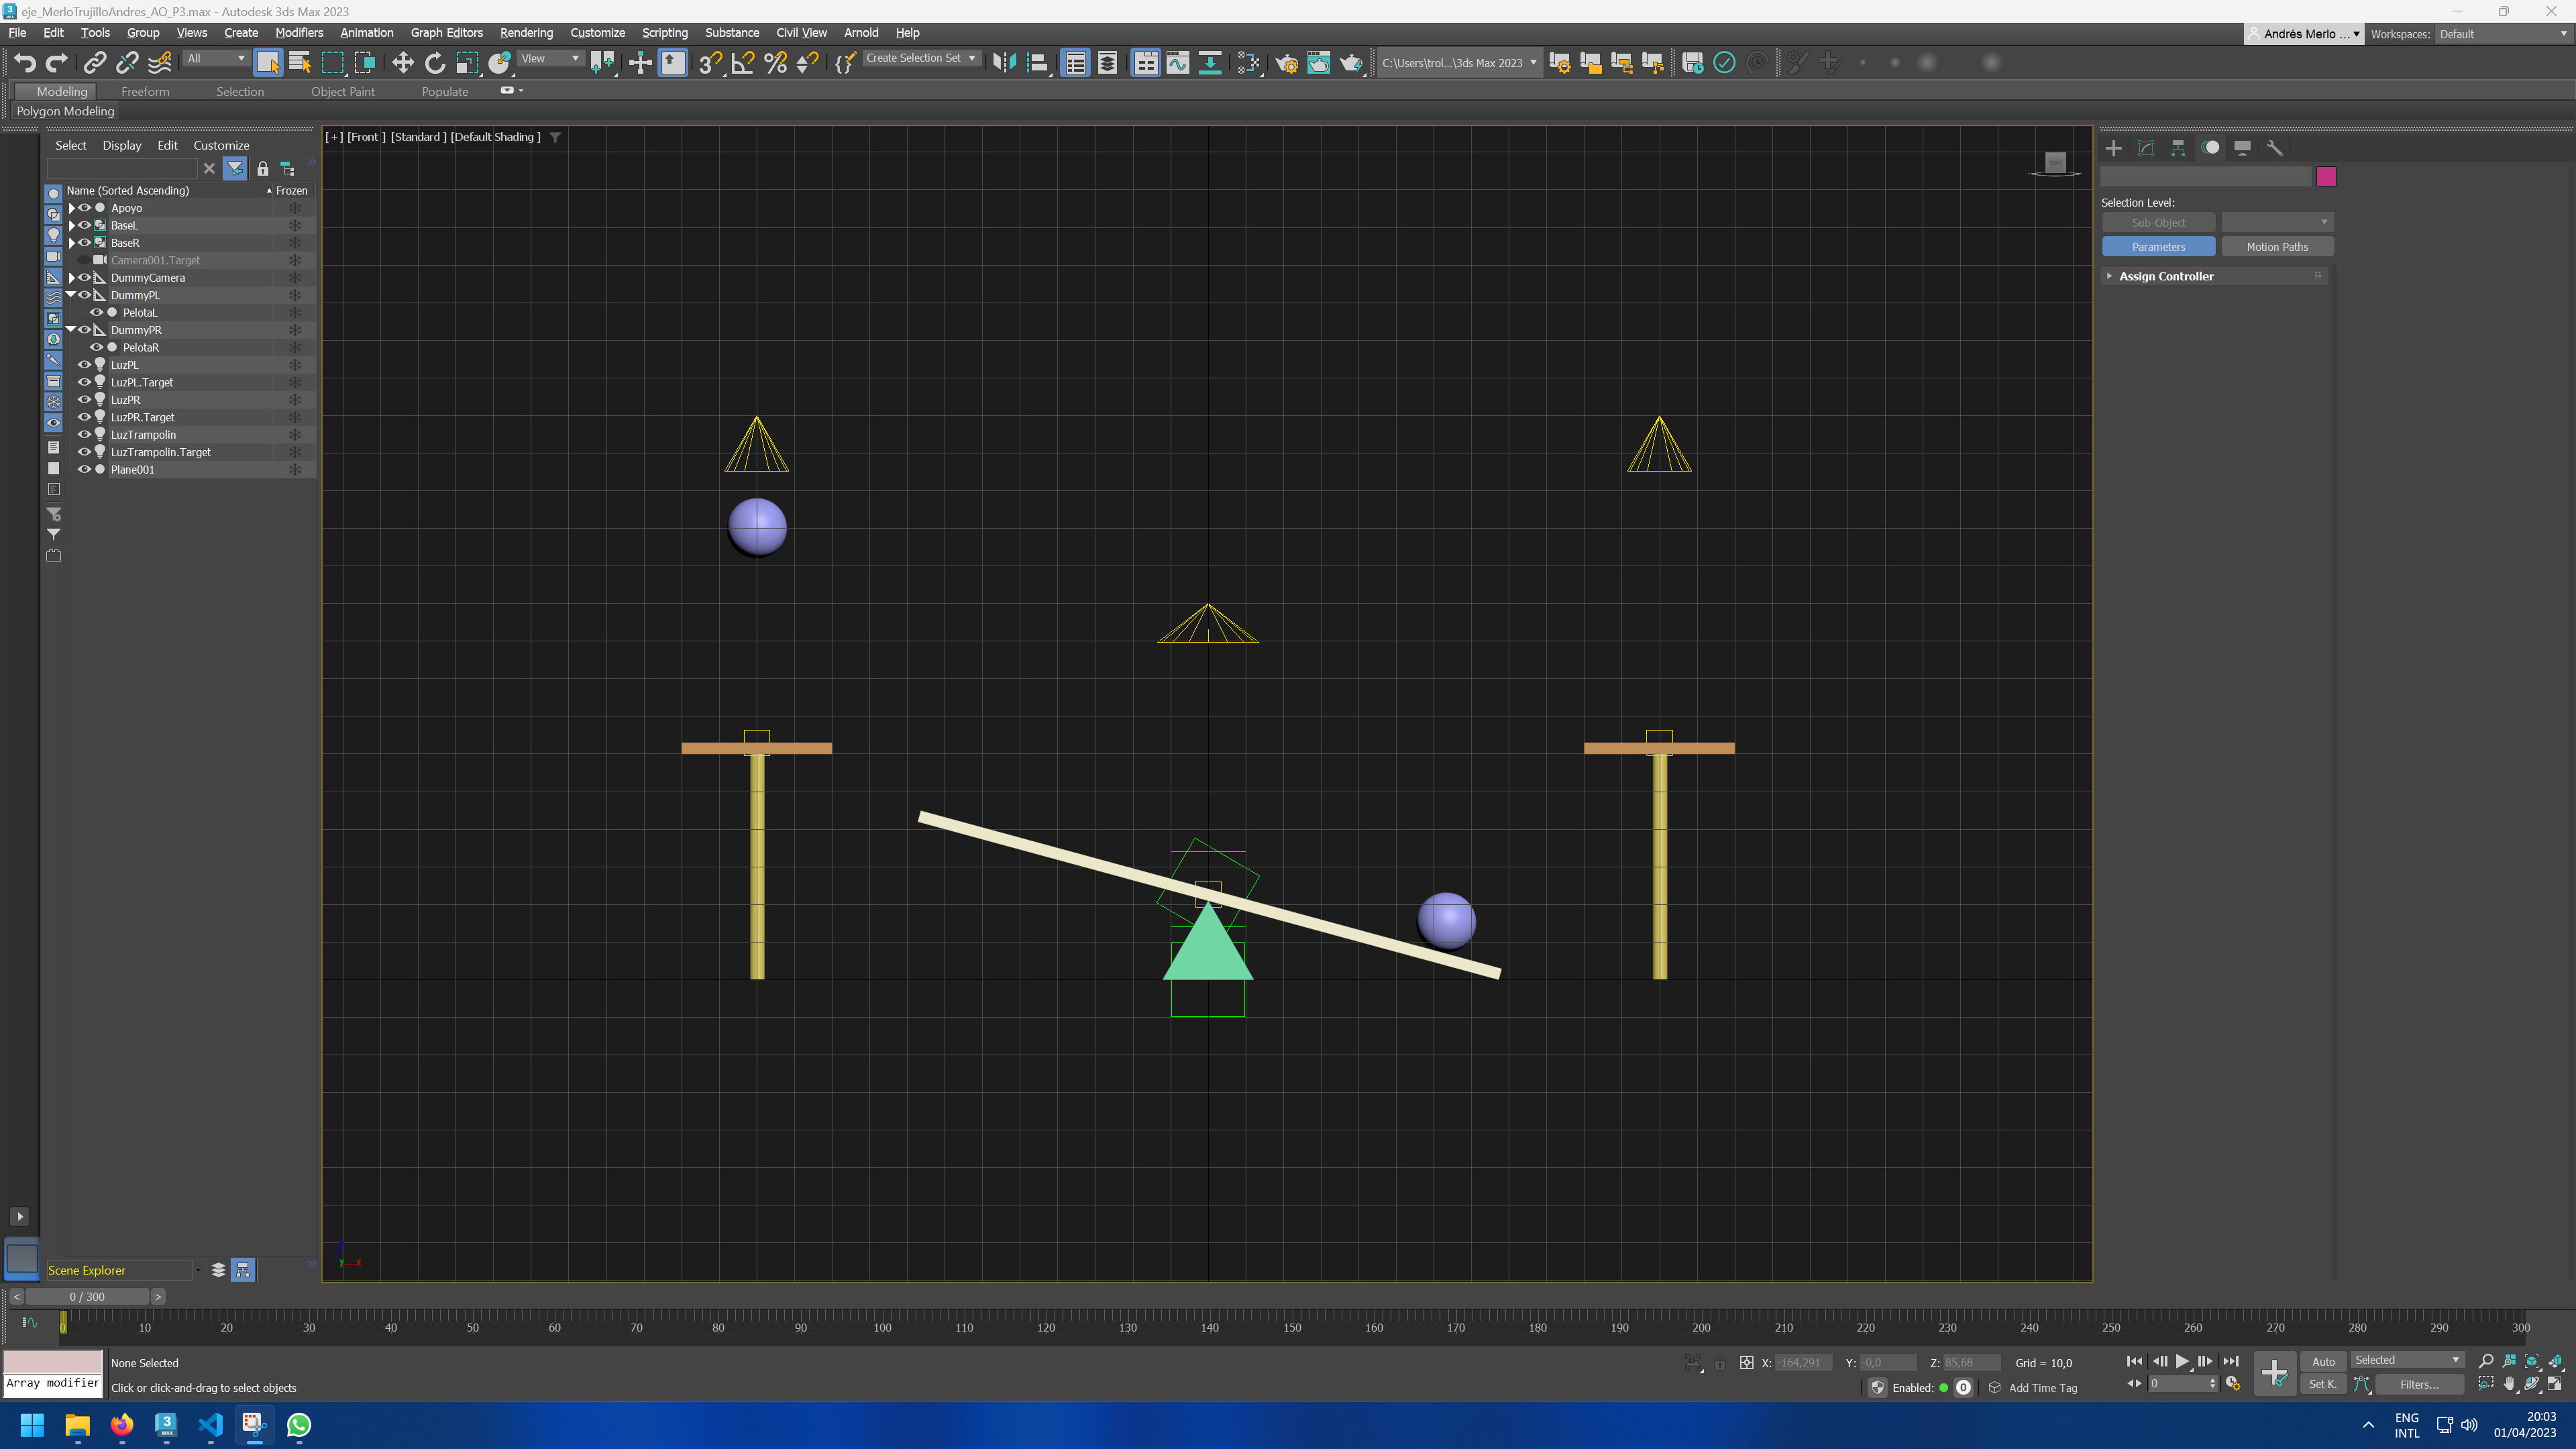
\includegraphics[width=\textwidth]{imagenes/Ejercicio 1/keyframes/0.png}
%         \caption{Pelotas en el instante 0.}
%     \end{subfigure}
%     \hfill
%     %\par\bigskip %si se desea dejar un margen entre la imagen de arriba y de abajo
% 	\begin{subfigure}[t]{0.48\textwidth}
% 	    \centering
% 	    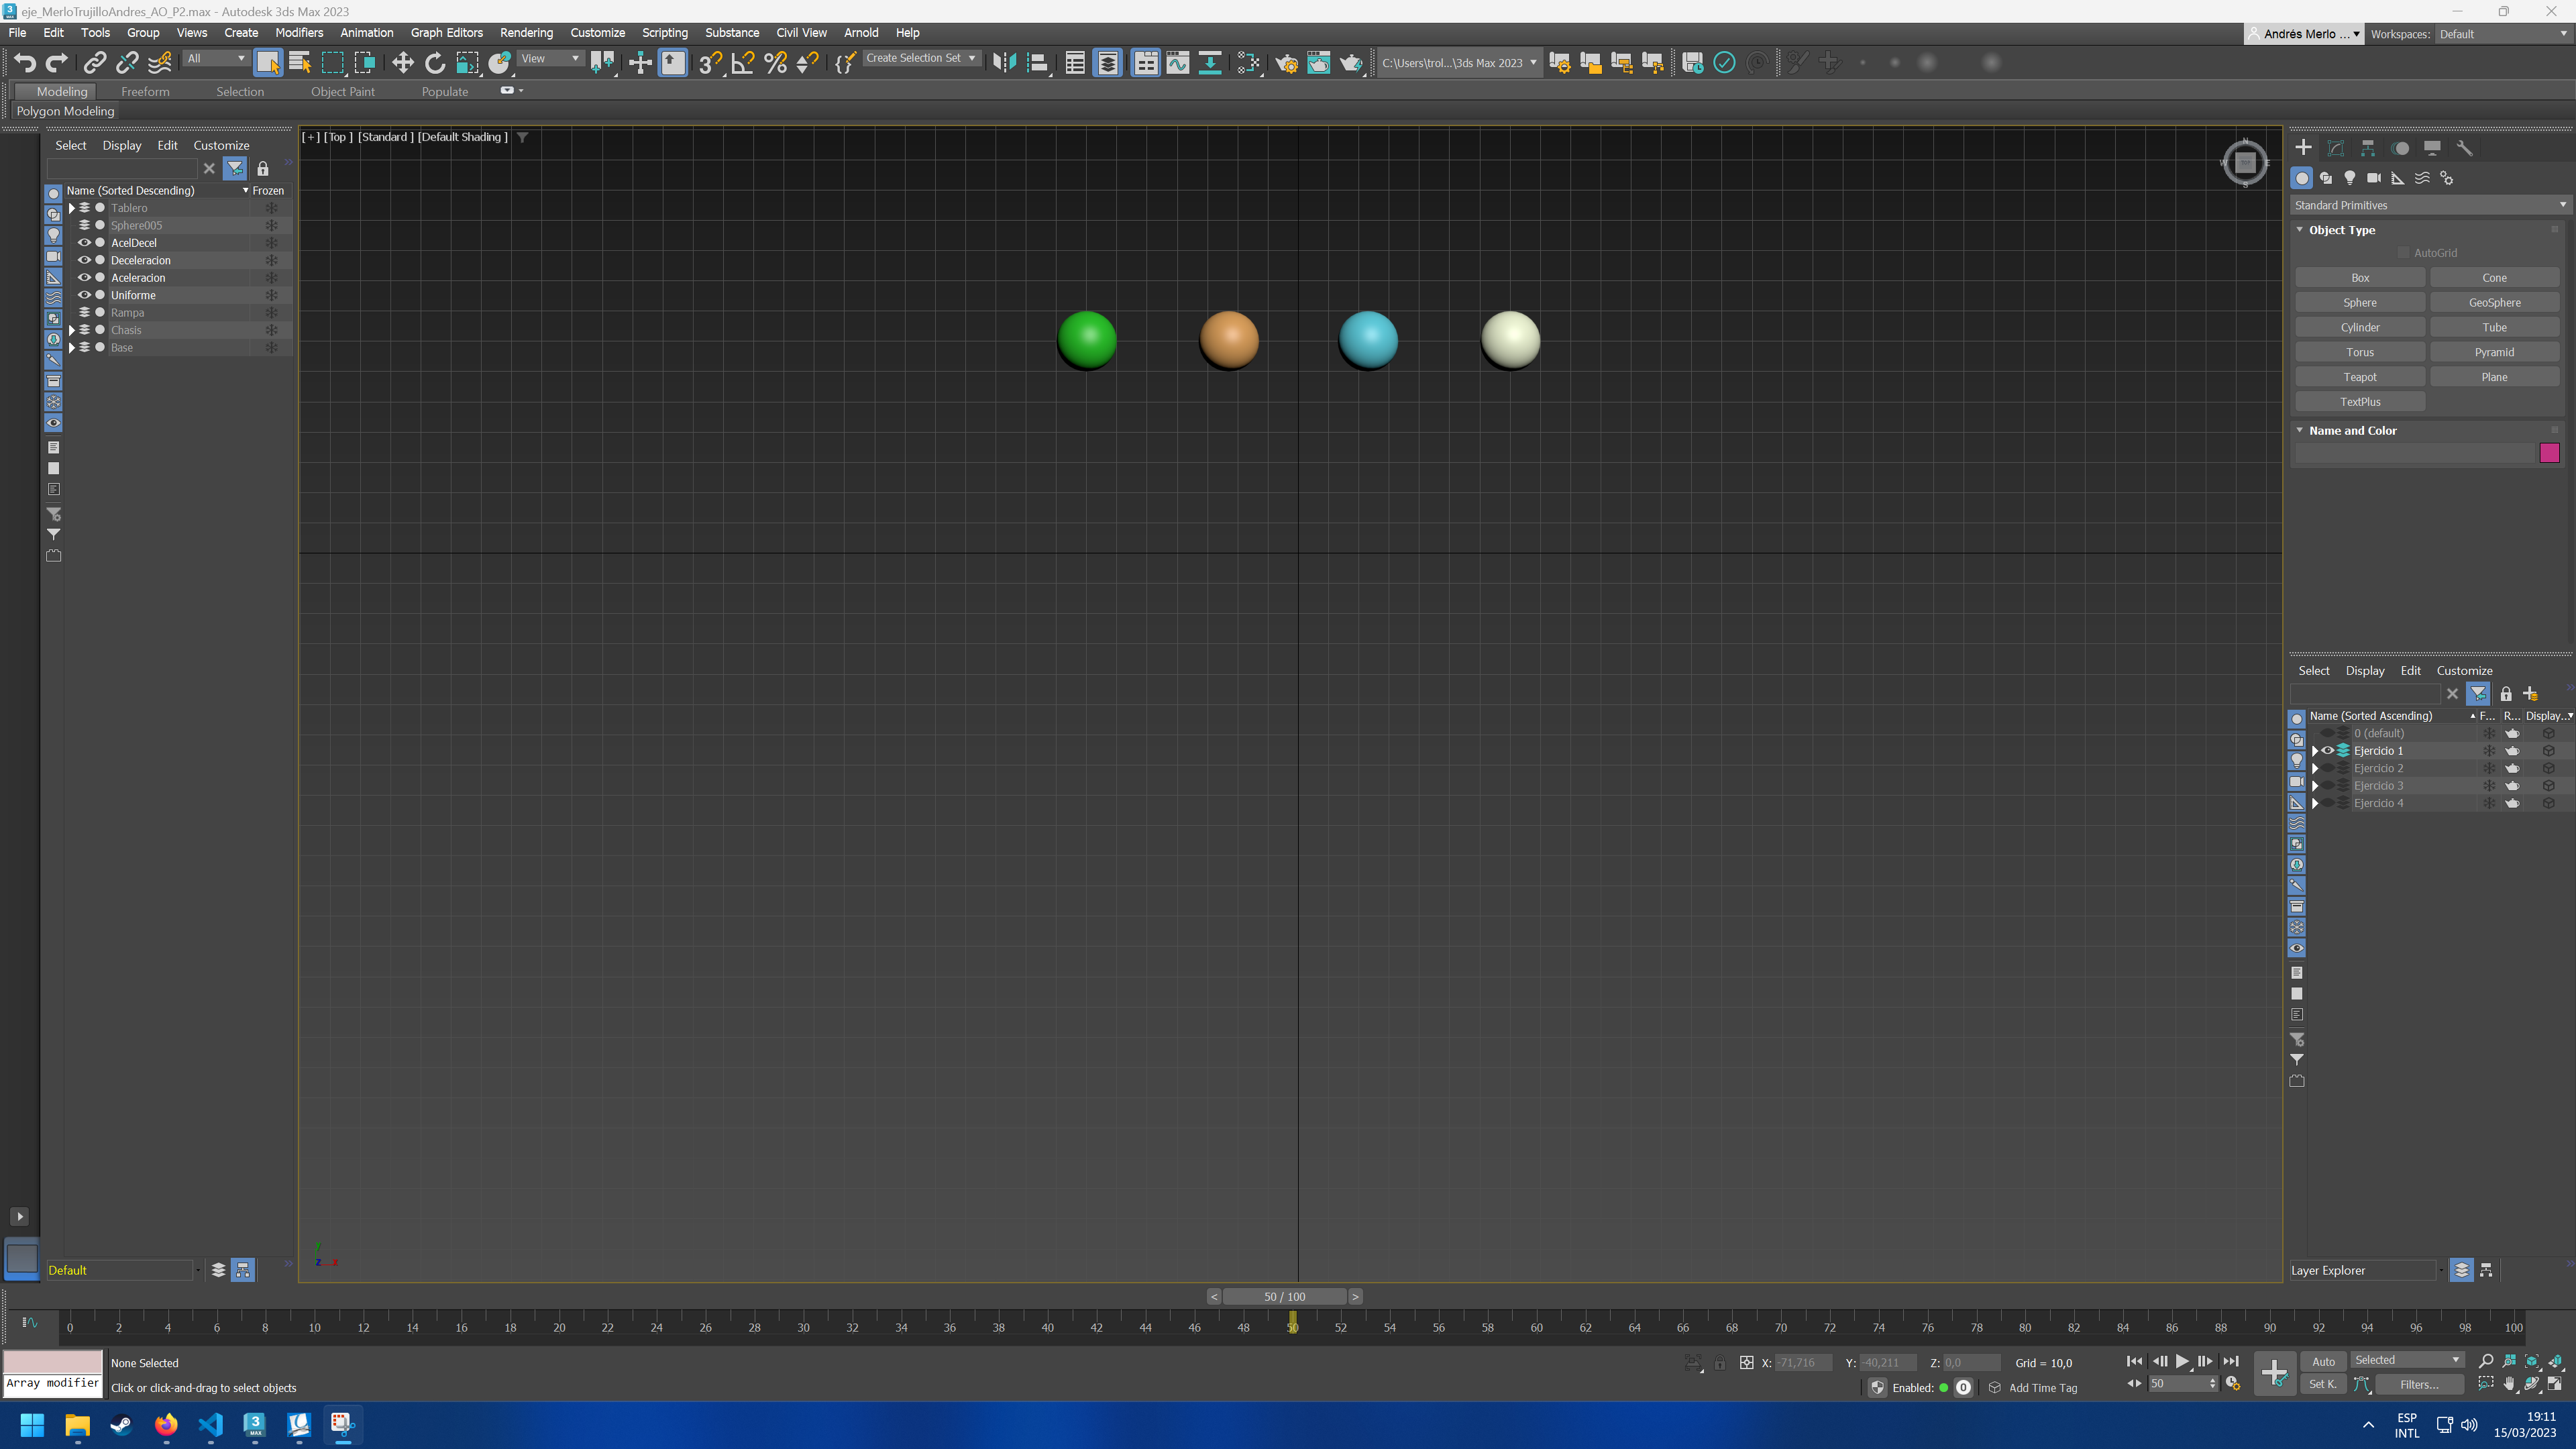
\includegraphics[width=\textwidth]{imagenes/Ejercicio 1/keyframes/50.png}
%         \caption{Pelotas en el instante 50.}
%     \end{subfigure}    
% \end{figure}


\section{Introducción}
% rescribir
En esta práctica se pide animar un conjunto de pelotas, que rebotan y caen a un balancín, haciendo que la otra rebote y caiga en una plataforma. También se debe animar un conjunto de luces que iluminará la parte de la escena que está en movimiento actualmente y una cámara, que rotará alrededor de la escena.

Todo lo mencionado anteriormente se debe \textit{loopear} de forma invertida, de manera que cuando acabe la animación vuelva a realizarse, pero al revés, comenzando por el final y acabando por el principio.

En esta memoria voy a dividir cada una de las partes que he realizado en secciones, las cuales se encontrarán a continuación.

\section{Número de fotogramas}

% rescribir
En la práctica se pedía que la animación durase 5 segundos, y otros 5 segundos haciendo la animación inversa. 

En mi caso, he usado 30 fotogramas por segundo, los que pone por defecto 3ds Max. Por tanto los cálculos para obtener lo números de fotogramas necesarios son los siguientes:


$30 \text{ fps} \times 2 \times 5 \text{ segundos} = 300 \text{ fotogramas} $

Cabe destacar que la animación debe acabar en el instante 150, para dar paso a su inversa y se complete.

\section{Composición de los objetos compuestos}

Los distintos objetos de la escena se han construido de la siguiente forma:

\begin{itemize}
    \item \textbf{Trampolín: }Se ha utilizado un cubo achatado y estirado para hacer la tabla y para el punto de apoyo se ha usado un cilindro con un circulo de 3 lineas, haciendo que sea un triangulo.
    
    Además, he modificado el pivote del tablero para que se encuentre justo en la unión del punto de apoyo con la tabla, para que gire de manera realista.

    Cabe destacar que he realizado una jerarquia en la que el punto de apoyo es el padre.

    \item \textbf{Bases: }Para las bases he utilizado un cubo achatado y un cilindro para el soporte, uniendo ambos en un grupo.
\end{itemize}


\section{Animación de la escena}

La animación la he realizado algo distinta a la que se pedía en el guion, ya que le comenté al profesor que el resultado era muy lento y me dijo que podía añadir algunos rebotes antes de comenzar la animación pedida. Para dar simetría, he animado dos rebotes al principio de la animación y al final. 

Además, como se pide seguir una forma Ping-pong cuando esté fuera de los \textit{keyframes} animados, va a haber \textit{keyframes} que se van a repetir en el instante 0 y 150; es decir, que no va a haber cambio con el siguiente o el anterior. Esto es necesario, ya que hay animaciones que no duran lo mismo, como el balancín, que su animación es más corta y si no se hiciera daría como resultado un giro prematuro del trampolin.

\bigskip

% rescribir
Para animar el movimiento de las pelotas que realizan en el balancín, he usado un objeto \textit{Dummy} con centro en la superficie del balancín y siendo padre de la pelota en la jerarquia; es decir, en la misma superficie donde las pelotas se encuentra.

% foto de los dummies

Además, para que la trayectoria que realicen no se vea afectada por la rotación del \textit{Dummy}, este se debe encontrar sin ninguna rotación en el momento en el que salen/entran al trampolín.

\bigskip

Ahora bien, como puede haber confusión sobre los distintos \textit{keyframes} para los objetos de la escena, voy a dividir cada objeto junto a su \textit{Dummy}, si lo tiene, en subsecciones:

\subsection{Pelota de la izquierda}

Los \textit{keyframes} para la pelota de la izquierda son:

\begin{itemize}
    \item \textbf{Instante 0: }La pelota se encuentra sobre su base, a cierta altura de la misma para realizar varios rebotes.
    \item \textbf{Instante 14: }La pelota se encuentra sobre su base, tocando la superficie de la misma, debido a la caida de la pelota.
    \item \textbf{Instante 26: }La pelota se encuentra en el aire, con la misma altura que en el instante 0. Esto lo hago asi para que la animación ping-pong funcione de manera mas o menos realista.
    \item \textbf{Instante 38: }La pelota se enceutnra sobre la superficie de la base, esta vez lista para saltar al trampolin.
    \item \textbf{Instante 48: }La pelota se encuentra en su punto mas alto del salto hacia el trampolin.
    \item \textbf{Instante 58: }La pelota ha caido y se encuentra sobre el trampolin.
    \item \textbf{Instante 150: }Exactamente igual que el instante anterior, para que la animacion se pueda rtepetir correctamente.
\end{itemize}

Los \textit{keyframes} para el \textit{Dummy} de la pelota de la izquierda son:

\begin{itemize}
    \item \textbf{Instante 0: }Se encuentra en su posición inicial, sin ninguna rotación para hacer que la trayectoria de la pelota sea correcta.
    \item \textbf{Instante 58: }Exactamente igual que el anterior \textit{keyframe}.
    \item \textbf{Instante 92: }El \textit{Dummy} se encuentra rotado hacia la izquierda, para animar el balanceo del balancin de manera correcta.
    \item \textbf{Instante 150: }Exactamente igual que el instante anterior, se hace para que la animación Ping-pong comienze al unísono con las demás.
\end{itemize}

Las curvas de la animación para el \textit{Dummy} son:

% curvas y explicacion

Y la trayectoria resultante es:

% fotos de la trayectoria resultante

\subsection{Pelota de la derecha}
Los \textit{keyframes} de la pelota de la derecha son:

\begin{itemize}
    \item \textbf{Instante 0: }La pelota se encuentra sobre la superficie del trampolín. Este instante solo es una extensión para que la animación ping-pong funcione correctamente y al mismo tiempo.
    \item \textbf{Instante 92: }Exactamente igual que el instante anterior.
    \item \textbf{Instante 102: }La pelota se encuentra sobre el punto más alto de la trayectoria hacia la base.
    \item \textbf{Instante 112: }La pelota ha acabado de realizar la trayectoria y se encuentra sobre la superficie de la base.
    \item \textbf{Instante 124: }La pelota se encuentra en el aire porque ha realizado un rebote.
    \item \textbf{Instante 136: }Ahora la pelota ha caido al suelo.
    \item \textbf{Instante 150: }Finalmente, la pelota da otro rebote y se encuentra en el aire de nuevo.
\end{itemize}

La curva de animación es:

% foto de la curva de animacion

Mientras que los \textit{keyframes} para su \textit{Dummy} son:

\begin{itemize}
    \item \textbf{Instante 0: }El \textit{Dummy} se encuentra rotado para que la pelota se encuentre sobre el tramploin. Al igual que con la pelota, se debe hacer para que la animacion inversa se haga al mismo tiempo.
    \item \textbf{Instante 58: }No ha habido cambios en la animación, es igual que el instante anterior.
    \item \textbf{Instante 92: }Ahora el \textit{Dummy} se encuentra rotado en la posición original; es decir, sin ninguna rotación aplicada para que la trayectoria de la pelota sea correcta.
    \item \textbf{Instante 150: }Ningún cambio realizado, solo es para que la animación inversa comience a la misma vez.
\end{itemize}

La curva de animacion para el \textit{Dummy} es:

% foto de la curva 


Y la trayectoria resultante es:

% foto de la trayectoria


% rescribir
Como se puede ver, esta pelota sigue el mismo espaciado de instantes que la otra, pero comenzando desde la derecha y sobre el trampolín, en vez de la izquierda. Esto hace que se pueda repetir la animación de manera sencilla, al ser simetricas dichas animaciones.
\subsection{Trampolín}


\subsection{Resultado final}

\section{Iluminación de la escena}

\section{Animación de la cámara}

\end{document}
